\chapter{Kubernetes}

Kubernetes is one of the most widely used container orchestration tools. Many cloud platforms provide Kubernetes support. Many opponent container orchestration tools are built on top of Kubernetes.

\section{Kubernetes Basics}

\textit{Kubernetes}, also known as \textit{k8s}, is an open-source container orchestration system originally developed by Google. It automates the deployment, scaling, and management of containerized applications. While Kubernetes is more flexible than Portainer, it's also more complex and has a steeper learning curve.

Notice that running Kubernetes on a local server differs significantly from running it on a cloud platform that often offers managed Kubernetes services with additional features and simplified managing interface. For example, AWS has EKS and Google cloud, Google Kubernetes Engine (GKE). Both of them have developed their own tools and interfaces for interacting with Kubernetes. So, while learning Kubernetes can be beneficial, one might not need to learn all the low-level details if he is using one of the above platforms instead of DIY everything.

The majority part of this chapter focuses on introducing running Kubernetes on a local server, in which case \textit{kubectl} is used as the user interface to Kubernetes and \textit{minikube} the software to manage the host machine. Minikube is an open-source software developed by the Kubernetes community to run a single-node Kubernetes cluster on a local machine, which is suitable for developers to learn and test different things in development environment.

Notice that in the past days, docker is the default container engine built-in to Kubernetes, and Kubernetes uses a special program ``dockershim'' to talk to the docker engine. As of now, docker support is deprecated in Kubernetes and dockershim is removed from the installation.

\subsection{Infrastructure}

Figure \ref{ch:vac:fig:kubernetescluster} demonstrates the key components Kubernetes has inside its cluster.
\begin{figure}[htbp]
	\centering
	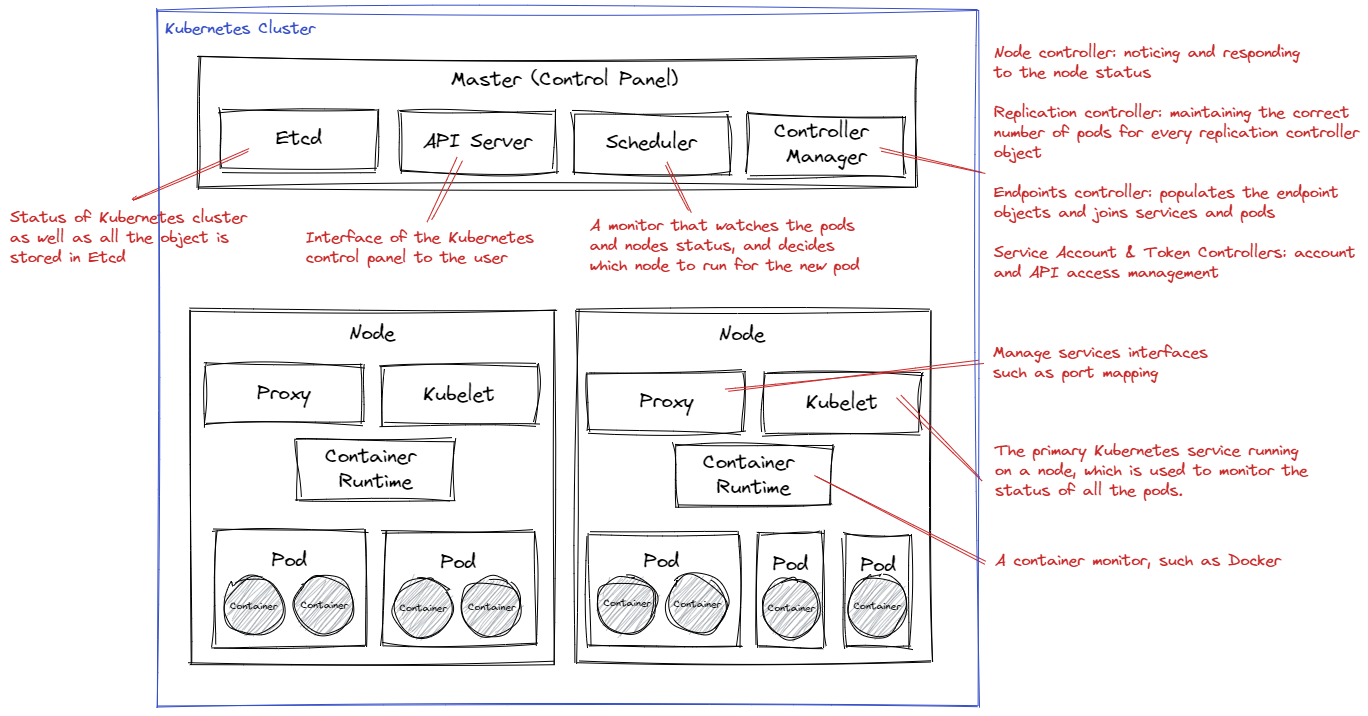
\includegraphics[width=350pt]{chapters/part-3/figures/kubernetescluster.png}
	\caption{Kubernetes cluster and its key components.} \label{ch:vac:fig:kubernetescluster}
\end{figure}
As shown in Fig. \ref{ch:vac:fig:kubernetescluster}, Kubernetes manages containers in a centralized ``master-worker'' manner, where the master plays as the control panel to interact with a user, and the worker nodes (nodes, for short) process the data. Each node can host multiple pods. Inside each pod is a container or a group of containers that work together closely (dependently, in many cases). Notice that in Kubernetes, containers never run directly in a node. They are always grouped into pods. A pod should be the minimal unit  that can deliver a basic function.

The master and nodes can run on cross servers or VMs. Kubernetes packages need to be installed on each and every server or VM. Kubernetes provides variety of tools to distribute the loads to different servers or VMs, or to add redundancy to the system for high availability.

\subsection{Installation}

The installation guidance of Kubernetes can be found at its official website \textit{kubernetes.io}. Notice that different OS adopts different ways of installing and using Kubernetes. The installation procedures introduced in this section applies to Linux OS only. For Windows users, Kubernetes can be installed from Docker desktop. For macOS users, other tools are used to install the tools.

As introduced earlier, \textit{kubectl} is used to interact with Kubernetes. In addition, since we are in development environment, we will also install \textit{minikube} which is used to setup a small Kubernetes cluster in the local machine. They can be installed separately. See following links for more details.
\begin{lstlisting}
https://kubernetes.io/docs/tasks/tools/install-kubectl-linux/
https://minikube.sigs.k8s.io/docs/start/
\end{lstlisting}
and do not forget to start \textit{minikube} using the following command. Notice that when both \textit{minikube} and \textit{kubectl} are installed, \textit{minikube} needs to be started before \textit{kubectl} can work properly.
\begin{lstlisting}
$ minikube start
\end{lstlisting}
Upon the start of \textit{minikube}, use the following command to verify the successful running of \textit{kubectl}.
\begin{lstlisting}
$ kubectl cluster-info
Kubernetes control plane is running at https://192.168.49.2:8443
CoreDNS is running at https://192.168.49.2:8443/api/v1/namespaces/kube-system/services/kube-dns:dns/proxy
\end{lstlisting}
Notice that when starting \textit{minikube}, it would launch a VM using Vertual Box, and install \textit{kubectl} as a built-in. Therefore, it is probable to use that built-in \textit{kubectl} instead of manually installing one separately. In that case, use the following command to verify the successful running of \textit{kubectl}
\begin{lstlisting}
$ minikube kubectl cluster-info
Kubernetes control plane is running at https://192.168.49.2:8443
CoreDNS is running at https://192.168.49.2:8443/api/v1/namespaces/kube-system/services/kube-dns:dns/proxy
\end{lstlisting}
in which case \verb|alias kubectl="minikube kubectl --"| may make things easier.

It is possible to run Kubernetes cluster directly on a host machine OS without VM if that machine is running Linux. However, this is not recommended for reasons pertaining to access control, security, and isolation. It is generally a better practice to deploy Kubernetes clusters in a VM.

The \verb|kubectl| command is a command-line interface (CLI) for interacting with Kubernetes clusters. Its behavior is governed by a configuration file, typically located at \verb|~/.kube/config|, which determines which Kubernetes cluster \verb|kubectl| communicates with. This could be a cluster running on the host machine, or a cluster running in a VM managed by tools like Minikube. 

\subsection{Kubernetes Configuration Files}

Kubernetes requires that all images to be used are pre-built. When using Kubernetes, multiple configuration files are required, each file corresponding with an object to be created. Notice that an object is not necessarily a container. It can be a pod, a replica controller, a service, or any item in the Kubernetes framework. There are manual setups of networking. Details are introduced in the remaining of this section.

The following two configuration files are given as examples to demonstrate how the configuration files of Kubernetes look like. This example comes from Udemy course \textit{Docker and Kubernetes: The Complete Guide} by Stephen Grinder \cite{stephen2023docker}. They are both written in YAML. Configuration file to setup a pod:
\begin{lstlisting}
apiVersion: v1
kind: Pod
metadata:
name: client-pod
labels:
component: web
spec:
containers:
- name: client
image: <image-name>
ports:
- containerPort: 3000
\end{lstlisting}
Configuration file to setup the networking service:
\begin{lstlisting}
apiVersion: v1
kind: Service
metadata:
name: client-node-port
spec:
type: NodePort
ports:
- port: 3050
targetPort: 3000
nodePort: 31515
selector:
component: web
\end{lstlisting}

Commonly used Kubernetes object types are summarized in Table \ref{ch:vac:tab:objtype}.
\begin{table}[htbp]
	\centering
	\caption{Commonly used Kubernetes object types.} \label{ch:vac:tab:objtype}
	\begin{tabularx}{\textwidth}{lX}
		\hline
		Object Type & Description \\
		\hline
		Pod & The smallest and most basic unit in the Kubernetes object model. It represents a single instance of a process running on the cluster. \\ \hdashline
		Deployment & Manages the deployment and scaling of a set of identical pods, ensuring the desired number of replicas are running and providing rolling updates for seamless application upgrades. \\ \hdashline
		Service & Enables network access to a set of pods using a stable IP address and DNS name. It provides load balancing across multiple pod replicas and allows external traffic to be directed to the appropriate pods. \\ \hdashline
		ConfigMap & Stores configuration data in key-value pairs, which can be consumed by pods as environment variables, command-line arguments, or mounted as files. \\ \hdashline
		Secret & Similar to a ConfigMap, but specifically designed to store sensitive data, such as passwords, API keys, and TLS certificates. Secrets are encrypted at rest and can be mounted into pods as files or exposed as environment variables. \\ \hdashline
		PersistentVolume & Provides a way to provision and manage persistent storage resources in a cluster. It decouples the storage from the underlying infrastructure and allows data to persist beyond the lifecycle of individual pods. \\ \hdashline
		PersistentVolumeClaim & Requests a specific amount of storage from a PersistentVolume. It acts as a request for a specific storage resource and provides an abstraction layer for managing persistent storage in a cluster. \\ \hdashline
		Ingress & Manages external access to services within a cluster. It acts as a reverse proxy and exposes HTTP and HTTPS routes to route traffic to the appropriate services based on hostnames, paths, or other rules. \\
		\hline
	\end{tabularx}
\end{table}
Some highlights of the above configuration files are as follows.
\begin{itemize}
	\item \verb|apiVersion| plays as the prefix that decides what configuration types are supported. For example, under the scope of \verb|v1|, \verb|Pod|, \verb|Service|, \verb|configMap|, \verb|Namespace|, etc., are supported. In a different \verb|apps/v1|, a different set of configuration types \verb|ControllerRevision|, \verb|StatefulSet|, etc., are supported. It's important to choose the correct apiVersion for the Kubernetes API version to ensure the compatibility and availability of the desired configuration options.
	\item \verb|kind| This indicates the type of the object that the configuration file describes. For example, \verb|Pod| represents a pod that is used to host containers, and \verb|Service| the primary object type that defines networking, with subtypes \verb|NodePort| (see example above), \verb|ClusterIP|, \verb|LoadBalancer| and \verb|Ingress|.
	\item \verb|metadata| indicates the name and labels of the object. For example, \verb|component: web| is defined as a label of the pod. This information is passed to the networking service under \verb|selector|, so that the networking service knows which object it should link to.
	\item \verb|port|, \verb|targetPort| and \verb|nodePort| are used to specify ports used in the service. The \verb|targetPort| indicates which port in the pod should be exposed to the service, and it is consistent with \verb|containerPort| defined in the pod. Assume that there is another pod in the node who needs to talk to this pod via the service. The other pod's port that communicates with the service is fed into \verb|port|. Finally, \verb|nodePort| is the port with value between 30000 and 32767 that is exposed from the service to outside the node. If \verb|nodePort| is not assigned, a random number within the range will be assigned. This is shown in Fig. \ref{ch:vac:fig:nodeport}.
\end{itemize}
Notice that Kubernetes networking using \verb|kind: Service| is more complicated than shown in the above example. More details of it is given later in a dedicated Section \ref{ch:vac:subsec:k8snetworking}.

\begin{figure}[htbp]
	\centering
	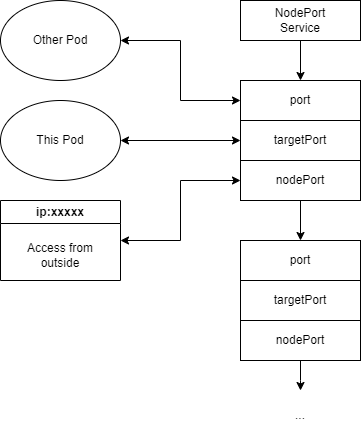
\includegraphics[width=200pt]{chapters/part-3/figures/nodeport.png}
	\caption{The NodePort networking service.} \label{ch:vac:fig:nodeport}
\end{figure}

\subsection{Cluster Deployment}

With the image and the configuration files ready, the next step is to deploy the nodes, pods, and containers. \textit{kubectl} command line interface is used to instruct Kubernetes to deploy the objects as follows.
\begin{lstlisting}
$ kubectl apply -f <configuration file>
\end{lstlisting}
This essentially asks the master node in the Kubernetes cluster to start taking actions according to the configuration files, such as to inform the nodes to start creating pods and containers. The master node also keeps monitoring the status of each work node, to make sure that everything is running as planned. If there is a container failure, etc., the master node will guide the associated note to restart the container.

It is worth mentioning here that by default Kubernetes uses declarative deployment instead of imperative deployment, meaning that the developer does not need to specifically tell Kubernetes what to do in each step. The developer only tells the overall objectives, and Kubernetes master node will try to figure out the steps to realize that goal. It is possible to enforce Kubernetes master node to practice specific details via configuration files, but it is almost always recommended to use the default declarative approach with Kubernetes.

To retrieve information, such as the status, of a group of objects, use
\begin{lstlisting}
$ kubectl get <object type>
\end{lstlisting}
where \verb|<object type>| can be \verb|pods|, \verb|services|, etc. For more details of a specific object, use
\begin{lstlisting}
$ kubectl describe <object type> <object name>
\end{lstlisting}
for example, to check the containers running in a pod. If \verb|<object name>| is neglected, Kubernetes returns detailed information of all objects of the given object type. For a running object, use
\begin{lstlisting}
$ kubectl logs <object name>
\end{lstlisting}
to check the log file of that object.

With the above been done, open a browser and use \verb|<ip>:<port>| to access the application running in the container, where \verb|<ip>| is the IP address of the VM (not \verb|localhost|) that \textit{minikube} created, and \verb|<port>| the port configured in NodePort service under \verb|nodePort|. The IP address can be found by running \verb|minikube ip|.

To apply a group of configuration files all together, provide the directory name of all the configuration files to Kubernetes instead of feeding each configuration file one at a time.
\begin{lstlisting}
$ kubectl apply -f <directory>
\end{lstlisting}
When directory is given instead of a file, Kubernetes will try to apply all the configuration files in that directory.

It is possible to consolidate the configuration files of objects into one conjunctive configuration file. To do that, use \verb|---| to split the configurations for each object in the conjunctive configuration file as follows. It is of personal preference whether to use conjunctive configuration files or separate configuration files for all objects.
\begin{lstlisting}
<configurations-for-object-1>
---
<configurations-for-object-2>
---
<...>
\end{lstlisting}

\subsection{Cluster Update} \label{ch:vac:subsec:updatek8s}

Without container orchestration tools such as Kubernetes, one of the most challenging tasks is to update the container for a different configuration, for example, changing the underlying image. With the help of Kubernetes declarative approach, it is possible update the cluster simply by revising the configuration files, and pass them to Kubernetes as if the cluster is to be deployed for the first time. Kubernetes automatically checks the names and kinds of the revised configuration files, comparing them with existing running objects, and update them if necessary.

Check the status of the pods using \verb|kubectl get pods|. After updating, the pods are often restarted, hence it is expected to see increment in the ``RESTARTS'' tag. To double confirm that updates have been made, use \verb|kubectl describe| to check the details of the relevant objects.

However, there is a limitation to the updating of the Kubernetes deployment. For an existing object, only certain fields in the configuration files can be changed. For example, for a pod that runs containers, the image can be changed, but the container port cannot. Sometimes there can be a walk around. For example, in the case of changing container port of pods, consider using a new object type \verb|Deployment| instead of \verb|Pod|, which allows more flexible updating. The \verb|Deployment| in its backend is consist of one or more monitored and managed identical pods.

To revert \verb|kubectl apply|, i.e., to remove a configuration file, use
\begin{lstlisting}
$ kubectl delete -f <configuration file>
\end{lstlisting}
Kubernetes treats the above delete command as a specific type of update to the cluster, and will action accordingly.

\section{Kubernetes Advanced}

This section introduces advanced commonly used Kubernetes objects, tools and techniques.

\subsection{Kubernetes Object: Deployment} \label{ch:vac:subsec:deployment}

As introduced in Section \ref{ch:vac:subsec:updatek8s}, updating pods has some limitations. It is practically more convenient to setup pods using ``Deployment'' object instead of ``pod''. The Deployment object servers as an additional layer of Kubernetes infrastructure that manages identical pods. More details of Deployment object is introduced in this section.

As an example, here is a configuration file from Kubernetes manual that deploys a Deployment object.
\begin{lstlisting}
apiVersion: apps/v1
kind: Deployment
metadata:
name: nginx-deployment
labels:
app: nginx
spec:
replicas: 3
selector:
matchLabels:
app: nginx
template:
metadata:
labels:
app: nginx
spec:
containers:
- name: nginx
image: nginx
ports:
- containerPort: 80
\end{lstlisting}
Some highlights are as follows.
\begin{itemize}
	\item \verb|replicas| gives the expected number of pods that the Deployment object manages.
	\item \verb|matchLabels| specifies the pods with which label are to be managed by the Deployment object. In this example, the label is \verb|app: nginx|. When populating pods, the pods would have the same label, as the same label is assigned under \verb|template|, \verb|metadata|, \verb|labels|.
	\item \verb|template| specifies the template that is used to create the pods.
\end{itemize}

When a new version of an image becomes available, we may want to update the containers accordingly. Re-apply the same configuration file would not help, as Kubernetes would reject apply request if no change is detected in the configuration file. It would not check whether the image is in its latest version. Kubernetes uses the following imperial command to update images as a walk around, and the developer needs to run this command manually.
\begin{lstlisting}
$ kubectl set image deployment/<Deployment name> <container name>=<image name>
\end{lstlisting}
For example,
\begin{lstlisting}
$ kubectl set image deployment/nginx-deployment nginx=nginx:1.25.1
\end{lstlisting}

\subsection{Kubernetes Object: Service} \label{ch:vac:subsec:k8snetworking}

There are 4 service types defined in Kubernetes. So far ``NodePort'' service type has been introduced in earlier examples. More types are introduced here.

A summary of different service types are given below.
\begin{itemize}
	\item ClusterIP: Exposes the service object on a cluster-internal IP. Objects in the cluster can access to the object that a ClusterIP is pointing at.
	\item NodePort: Assigns a static port with the cluster IP, and exposes the Service object to the internet. This is used mostly used in development environment, not in production environment.
	\item LoadBalancer: Exposes the service object externally using an external load balancer. Kubernetes does not provide built-in load balancer.
	\item ExternalName: Maps the service object to the contents of the \verb|externalName| field, such as a host name. This is related to cluster DNS server.
\end{itemize}

\vspace{0.1in}
\noindent \textbf{ClusterIP}
\vspace{0.1in}

A ClusterIP configuration file may look like the following.
\begin{lstlisting}
apiVersion: v1
kind: Service
metadata:
name: client-cluster-ip-service
spec:
type: ClusterIP
selector:
<target tag>
ports:
- port: <port for internal comm>
targetPort: <port for internal comm>
\end{lstlisting}
where the first \verb|port for internal comm| is the port in the ClusterIP service object that opens to other objects in the cluster, and the second the port the target object opens to the ClusterIP service object. They can be set differently, but usually they are just set to the same value.

\vspace{0.1in}
\noindent \textbf{NodePort}
\vspace{0.1in}

NodePort has already been introduced earlier. It exposes the object to the internet with a static port, and it is used more in a development environment than a production environment.

\vspace{0.1in}
\noindent \textbf{LoadBalancer}
\vspace{0.1in}

LoadBalancer is a legacy way of getting network traffic into the pods. It is essentially an interface or a tool to bridge an Kubernetes Deployment with an external load balancer. It will try to automatically configure the external load balancer using the configuration provided by the developer, while compromising the external load balancer rule.

\vspace{0.1in}
\noindent \textbf{Ingress}
\vspace{0.1in}

Ingress is a more commonly used Service type than LoadBalancer to get traffic into the Kubernetes containers. There are different types of Ingress, for example, Nginx Ingress by \textit{github.com/kubernetes/ingress-nginx}. A demonstrative example of ingress service realization is given in Fig. \ref{ch:vac:fig:ingress_service}. In this implementation framework, the configuration file (mainly a set of routing rules) of the object is used to define an ``Ingress Controller'' which manages the runtime that controls inbound traffic. In some applications such as \textit{kubernetes/ingress-nginx}, the ingress controller and the runtime are integrated together.

\begin{figure}[htbp]
	\centering
	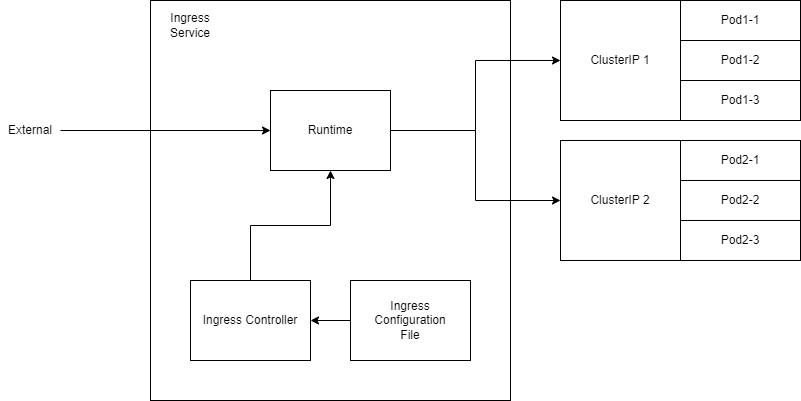
\includegraphics[width=350pt]{chapters/part-3/figures/ingress_service.png}
	\caption{An example of ingress service framework.} \label{ch:vac:fig:ingress_service}
\end{figure}

The ingress configuration differs depending on the ingress service type and the platform. Details are not given here.

\subsection{Kubernetes Object: Persistent Volume Claim, Persistent Volume, and Volume} \label{ch:vac:subsec:k8svolume}

Docker engine uses volumes to maintain persistent data and share data among containers. Details have been introduced in Section \ref{ch:vac:subsec:dockervolume}. Kubernetes volume framework is similar in the sense that it makes sure that the data is saved and managed by the host machine, so that when the pods or containers are shutdown or restarted, the data can be restored safely.

Do notice that when comes to data sharing using volume, it is dangerous to have multiple containers or the host machine accessing the same files simultaneously, without knowing the existence of each other. Usually additional steps need to be setup to ensure data consistency.

It is worth emphasizing the differences of ``volume'' technology in containerization and Kubernetes volume-related objects: Persistent Volume Claim (PVC). Persistent Volume (PV), and Volume. As a matter of fact, Kubernetes Volume object is usually not what we want. Kubernetes Volume creates the volume tied to a pod, not to the host machine. It survives container failure in the pod, but not pod failure. In summary:
\begin{itemize}
	\item Kubernetes Volume: A volume tied to the pod. It survives container failure inside the pod, but not pod failure.
	\item Kubernetes PV: A volume tied to the host machine. It survives pod failure. It can be provisioned either automatically by a StorageClass, or manually by the developer and administrator.
	\item Kubernetes PVC: It is essentially a request sent from a pod or a container, asking for specific amount of storage from a PV. Kubernetes will find that amount of PV from either existing provisioned static PV, or dynamically provision new ones for the pod or container.
\end{itemize}
Notice that it is not necessary to claim PV in order to use PVC, as PVC can provision PV dynamically. There is a one-to-one relationship between the provisioned PV and the PVC. If there are multiple pods, each requiring a dedicated PV, then multiple PVCs must be used. The developer can either create those PVCs manually, or use a Volume Claim Template to claim them if they are similar.

An example of claiming Kubernetes PV and PVC is given below. In the remaining part of this section, we will be mostly using PVC instead of PV.
\begin{lstlisting}
# persistent-volume.yaml

apiVersion: v1
kind: PersistentVolume
metadata:
name: my-pv
spec:
storageClassName: standard
capacity:
storage: 10Gi
accessModes:
- ReadWriteOnce
hostPath:
path: /data/my-pv
---
# persistent-volume-claim.yaml

apiVersion: v1
kind: PersistentVolumeClaim
metadata:
name: my-pvc
spec:
storageClassName: standard
accessModes:
- ReadWriteOnce
resources:
requests:
storage: 5Gi
\end{lstlisting}
To check the PV objects, use \verb|$ kubectl get pv| and \verb|$ kubectl get pvc|.

To add the above Kubernetes PVC to a Kubernetes Deployment, add volumes information to the specs as given in the following example.
\begin{lstlisting}
apiVersion: apps/v1
kind: Deployment
metadata:
name: my-app-deployment
spec:
replicas: 1
selector:
matchLabels:
app: my-app
template:
metadata:
labels:
app: my-app
spec:
containers:
- name: my-app-container
image: my-app-image
ports:
- containerPort: 8080
volumeMounts:
- name: data-volume
mountPath: /data
subPath: data-from-container
volumes:
- name: data-volume
persistentVolumeClaim:
claimName: my-pvc
\end{lstlisting}
where \verb|volumes| defines which Kubernetes PVC is used, and \verb|volumeMounts| tells how it is mounted in the container. The \verb|mountPath| is the path in the container whose data is mounted by the volume. If a \verb|subPath| is given, a sub-folder of its specified name will be created in the host machine in the volume to contain the data.

There are different types of access modes:
\begin{itemize}
	\item \verb|ReadWriteOnce|: Allow one node to read and write at a time.
	\item \verb|ReadOnlyMany|: Allow many nodes to read at a time.
	\item \verb|ReadWriteMany|: Allow many nodes to read and write at a time.
\end{itemize}

The developer can specify the place for Kubernetes PVs. This is usually the hard drive on a local server, a virtual storage space in the VM. Use the following command to check Kubernetes possible choice of storage.
\begin{lstlisting}
	$ kubectl get storageclass
\end{lstlisting}
and
\begin{lstlisting}
$ kubectl describe storageclass
\end{lstlisting}
When deploying Kubernetes on the Cloud, the developer needs to do additional configurations as there would be many storage options. Usually, each Cloud provider will have its own default storage space for Kubernetes, such as AWS Elastic Block Store for AWS.

\subsection{Kubernetes Object: Secrets} \label{ch:vac:subsec:k8ssecrets}

Kubernetes Secrets object is used store confidential information, such as the database password, API key, etc. It is often a piece of information that is necessary for the containers, but the developer does not want to present as plain text in the configuration file.

Secrets are not created from configuration files, which is the recommended way of creating other Kubernetes objects. Instead, it is created from one-time imperative command, inside which the confidential information needs to be told to Kubernetes. Use the following command to create a Secret object.
\begin{lstlisting}
$ kubectl create secret <type-of-secret> <secret-name> --from-literal <key>=<value>
\end{lstlisting}
There are 3 types of Secrets: \verb|generic|, \verb|docker-registry| and \verb|tls|.

\subsection{Kubernetes Environment Variables}

Kubernetes environment variables are used to pass or share information among Deployments. Depending on the features of the information, such as whether it is a constant global configuration or a dynamic value, whether it is plain text or confidential encoding, etc., it might be handled differently.

To define constant environment variables in containers, simply specify them in the Deployment configuration file as given in the example below.

\begin{lstlisting}
apiVersion: apps/v1
kind: Deployment
metadata:
name: my-app-deployment
spec:
replicas: 1
selector:
matchLabels:
app: my-app
template:
metadata:
labels:
app: my-app
spec:
containers:
- name: my-app-container
image: my-app-image
ports:
- containerPort: 8080
volumeMounts:
- name: data-volume
mountPath: /data
subPath: data-from-container
env:
- name: <name1>
value: <value1>
- name: <name2>
value: <value2>
- name: <name3>
valueFrom:
secretKeyRef:
name: <secret-name>
key: <key>
volumes:
- name: data-volume
persistentVolumeClaim:
claimName: my-pvc
\end{lstlisting}
where a new tag \verb|env| is defined under template, specifications, containers. Under the \verb|env| tag, a list is defined containing names and values of the environment variables. The value must be a string, not a numerical number.

\section{Kubernetes Deployment in Production Environment}

With the tools and methodologies introduced so far, we are able to deploy containers in development environment. This is good enough for testing purpose or for small individual projects. However, when comes to enterprise tier projects or collaborative projects, there is often a CI/CD pipeline that standardize the integration and delivery of the containers in production environment. Container orchestration tools such as Kubernetes is often a must have.

This section briefly introduces the steps to develop and deploy containers in production environment with Kubernetes. Figure \ref{ch:vac:fig:prodenvworkflow} gives an example of overview of what such deployment may look like. Notice that this example is more towards a community project but not an enterprise project.

\begin{figure}[htbp]
	\centering
	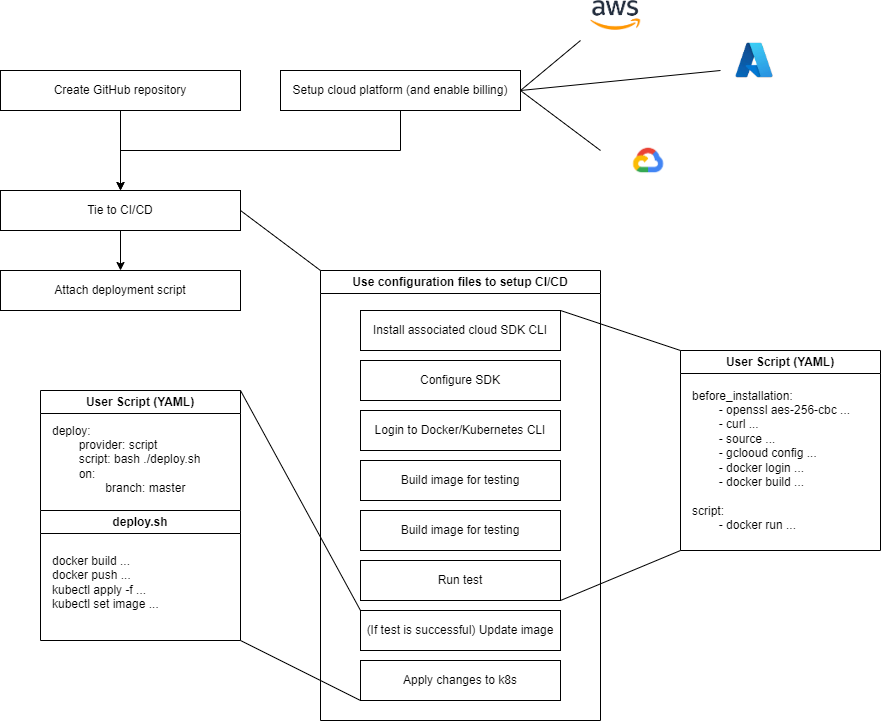
\includegraphics[width=350pt]{chapters/part-3/figures/prodenvworkflow.png}
	\caption{An example workflow of creating a production environment with Kubernetes.} \label{ch:vac:fig:prodenvworkflow}
\end{figure}

The example used in this section to demonstrate Kubernetes CI/CD on a cloud platform in production environment is taken from \cite{stephen2023docker}. Following \cite{stephen2023docker}, Google Cloud Platform is used as the cloud platform provider.

\subsection{Setup Cloud Account}

Many cloud platforms nowadays have a very good support of Kubernetes. The deployment of containers using Kubernetes can be done via their UIs easily. The developer needs to decide the resources to be used for the deployment. The more nodes and more power machine, the higher the charge. In most cases, the developer does not need to start a VM and install Kubernetes on it by himself. The cloud provider shall have dedicated Kubernetes engine service that would automatically configure the VM per required.

\subsection{Configure CI/CD}

Travis CI is a continuous integration service tool written. It can be deployed on the cloud and linked to a Github repository and a CI/CD platform such as a Kubernetes cluster on Google Cloud Platform.

To run Travis, a machine supporting Ruby programming language is required. For that, a separate container with Ruby installation is deployed to run Travis. Use Github credentials to login to Travis, so that it can link to the Github repositories.

Travis has built-in file encryption function. This function is mainly used to encrypt login credentials and service account credentials (in this example, the service account information to link to Kubernetes clusters on Google Cloud Platform) locally, so that later the unencrypted original credential files can be deleted, and only the encrypted credentials uploaded to the Github repository. When encrypting a file, Travis will also guide the user on how to call the encrypt information in the build script.

Travis uses configuration files to setup CI/CD pipeline.

\subsection{Deploy Containers}

In the Travis configuration file, \verb|deploy| is used to specify the script to run when the testing is successful. A separate bash script \verb|deploy.sh| is defined for this purpose, inside which is a sequence of commands that builds and publishes images, and configures Kubernetes using \verb|kubectl|.

It is particularly worth mention that in \verb|deploy.sh|, when building and applying the latest version of the docker image, tagging using \verb|<image-name>:latest| alone is not going to work for the same reason explained earlier in Section \ref{ch:vac:subsec:deployment}: when the same configuration with \verb|<image-name>:latest| is applied, the system would simply acknowledge it as ``no change'' and would not actually download the latest version of the image.

The walk around introduced in Section \ref{ch:vac:subsec:deployment} was to use version number in the configuration file and/or as an imperial command as follows.
\begin{lstlisting}
$ kubectl set image deployment/<Deployment name> <container name>=<image name>:<version>
\end{lstlisting}
so what when the version name changes, Kubernetes would notice the differences and apply the new image. When working with CI/CD using \textit{Git}, this can be further automated. Just use the \verb|$GIT_SHA| as part of the tag as follows.
\begin{lstlisting}
$ docker build -t <docker-id>/<image-name>:latest -t <docker-id>/<image-name>:$GIT_SHA -f <dockerfile> <save-directory>
$ docker push <docker-id>/<image-name>:latest
$ docker push <docker-id>/<image-name>:$GIT_SHA
\end{lstlisting}
Notice that in addition to \verb|:latest|, \verb|:$GIT_SHA| is used as a secondary tag. When pushing the built image to Docker Hub, both \verb|:latest| and \verb|:$GIT_SHA| are pushed (although they have identical content). When setting image, the \verb|$GIT_SHA| is used to identify the image just like the version number.

It is recommended not to remove \verb|:latest| in the building command. This is because if someone wants to pull and test the latest image in his server (without knowing the value of \verb|$GIT_SHA| for the latest commit), he is still able to do so using only the image name.

Notice that \verb|$GIT_SHA| is not a built-in environment variable. The developer needs to set that environmental variable manually in the configuration YAML file as follows. It is possible to replace \verb|$GIT_SHA| with a different name.
\begin{lstlisting}
env:
global:
- GIT_SHA=$(git rev-parse HEAD)
\end{lstlisting}
With the above setup, \verb|$GIT_SHA| can be used in \verb|deploy.sh| as an environmental variable.

\subsection{Manage Secrets}

Notice that when CI/CD tool is tied to the cloud platform provider, service account authentication is required. It is a good habit to NOT to put the authentication information in the CI/CD configuration file as plain text, or to upload the unencrypted file that contains the authentication information to the public workspace. It is possible that some CI/CD tools provide encryption tools that can be used to encrypt the authentication file. In such case, the developer may need to install the required CLI for that CI/CD tool.

In Section \ref{ch:vac:subsec:k8ssecrets}, it has been introduced that Kubernetes uses Secrets object to encrypt secret files. The encrypted secret files can then be safely published online. In the Kubernetes configuration file, an environmental variable can be created to call the secret information.

Many cloud platform providers including Google Cloud Platform provides services to manage secrets.

\subsection{Helm}

To install a software in a Kubernetes pod, the most intuitive way is to commit the installation in the image, and call the image in the Kubernetes configuration file. For commonly used services such as \verb|ingress-nginx|, its installation configuration file is available online as part of the manual. It essentially starts and initializes a branch of Kubernetes objects to enable the service.

Helm is designed as an alternative to manage software installation in Kubernetes clusters. In many occasions, it is more convenient (or even only possible) to use Helm to install a software. More details are given in \textit{github.com/helm/helm}.

We need to first install Helm from script. Helm installation used to contain two parts, the CLI (referred as Helm client) and the server (referred as Tiller server). We could then use Helm CLI to install other third-party software and tools.

Access control is important on cloud platforms. In practice, user accounts are used to identify users, and service accounts to identify pods and programs. Associated role bindings are used to manage what resources can be accessed by a user or program. For example, administrative role over the entire account can be used to bind with the administrative user. The same applies to Helm. The Tiller server required some extent of administrative control over the resources in an account. In many occasions, Tiller server was given the administrative permission to access the entire account, which introduced security risks.

As of Helm version 3, a major change was carried out where Tiller server was removed completely. Helm architecture is more secure and simpler today. The concerns related to Tiller's permission in the Kubernetes cluster are no longer relevant. Helm 3 of course requires permissions to use the resources, which is now managed by Kubernetes role-based access control mechanisms.
